\documentclass[11pt]{article}

\usepackage{amsmath}
\usepackage{textcomp}
\usepackage[top=0.4in, bottom=0.5in, left=0.4in, right=0.4in]{geometry}
% Add other packages here %
\usepackage{subcaption}
\usepackage{float}
\usepackage{wrapfig}
\usepackage{graphicx}
\usepackage{xcolor}


% Put your group number and names in the author field %
\title{\bf Excercise 1.\\ Implementing a first Application in RePast: A Rabbits Grass Simulation.}
\author{Group \textnumero 10: Cosmin-Ionut Rusu, Sorin-Sebastian Mircea}

\begin{document}

\maketitle

\section{Implementation}


We followed the provided tutorial which served as a base for our implementation. We carefully adopted the architecture described in the RePast tutorial and implemented the other requirements to fit our specific problem requirements. We've also followed Object-Oriented Programming principles as guidelines for the project.

\subsection*{Visualization}

In our graphical visualization of the simulation, the grass is coded with the green color, and the rabbits are coded with red, for best contrast. Empty cells are represented by black.

\begin{figure}[H]
\includegraphics[width=0.25\textwidth]{_world.png}
\centering
\label{fig:world}
\caption{Simulation world}
\end{figure}

\subsection*{Charts}
To better visualise and understand the world we have created two charts:

\begin{enumerate}
\item Showing the evolution of the grass available in the world and the population of rabbits. The rabbit population is multiplied by a constant (in our case 100) to bring them to similar scales.

\item  Histogram of the rabbits energy at the current step
\end{enumerate}

\subsection*{Extra parameters}
We considered that the the the following parameters would need to be added (besides the already provided ones) in order to have a better control of the world:

\begin{itemize}
\item \textbf{EnergyLostByMoving} - the energy that a rabbit is going to loose for moving;
\item \textbf{EnergyLostByReproduction} - the energy that a rabbit is going to loose in order to reproduce (once it reaches the reproduction threshold);
\item \textbf{MinRabbitInitEnergy} and \textbf{MaxRabbitInitEnergy} - rabbits are randomly going to receive a value from the interval as initial energy.
\end{itemize}

\subsection{Assumptions}
% Describe the assumptions of your world model and implementation (e.g. is the grass amount bounded in each cell) %

\subsection* {Actions order}
The order in which our world is going to execute the possible actions can have an impact on the outcome (even thought this is negligible). Arbitrarily we chose the following order (that is executing during one step):

\begin{enumerate}
\item  Move agents
\item  Agents eat (if they are on a grass)
\item  Agents loose energy
\item  Agents die (if energy = 0)
\item  Agents give birth (if $energy \geq birthThreshold$)
\item  New grass tiles are spawned
\end{enumerate}

\subsection* {Grass spawning}

Grass tiles cannot collide with other grass tiles (during spawning). Grass can be spawned on top of a rabbit but it will be consumed instantly by the rabbit.

We had to decide if we were going to spawn the grass only on the tiles that are unoccupied by the rabbits, or randomly everywhere. We chose the second one. When this happens, the rabbits are instantly going to benefit by the extra food, allowing them a second change before they might die. We believe this simulates a real life environment where rabbits can eat grass grown overnight.

\subsection* {Initial energy levels}
We also make sure that the initial energy level is always below the $birthThreshold$. This is a fair assumption since if a rabbit were to be born with an $energy level \geq birthThreshold$, then it might reproduce right away and we will have more rabbits than we expected (set by $numInitRabbits$ variable).

\subsection* {Rabbit in impossibility of movement}

In the case that a rabbit cannot move due to it being surrounded by other rabbits, we chose for the rabbit to stay on place but still loose energy (as a penalty for not being able to search for food).

\subsection* {Collision system}

Rabbits cannot collide with other rabbits (during spawning and movement), it can move onto a grass tile (and at that moment the grass will be consumed). A drawback on this iterative process is that the order in which we move the rabbits have an impact on the possibility of the movements of the individual rabbits. For example, if two rabbits were next to each other, after one of them moves, the other one will now be able to move to the position where the first one was initially. We assumed we always move the agents in the order the were generated.

\subsection{Implementation Remarks}
% Provide important details about your implementation, such as handling of boundary conditions %

\subsection* {Movements}

For moving the rabbits one step in the 4 adjacent cells, we defined two constant delta vectors. The first vector tells the change of the x position $dx = [0, 1,  0, -1]$ and the second vector tells the change of the y position $dy = [1, 0, -1,  0]$. We believe this is a very elegant solution and in order to make a legal move we first draw a random integer $d$ in [0, 3] and then use the following formulas to update the directions:

\begin{gather*} 
newx = (x + dx[d] + N) \% N \\
newy = (y + dy[d] + M) \% M
\end{gather*}

Where $N$ and $M$ are the number of rows and the number of columns the matrix, respectively. This formula takes care of all the corner cases and will make the space behave like a torus.


\section{Results}
% In this section, you study and describe how different variables (e.g. birth threshold, grass growth rate etc.) or combinations of variables influence the results. Different experiments with different settings are described below with your observations and analysis

Unless otherwise stated, the value of each variable is the default one depinted in the table \ref{table:constants}.

\begin{table}[h!]
\centering
\begin{tabular}{||c c||} 
 \hline
 Parameter & Default Value \\ [0.5ex] 
 \hline\hline
  GridSize & 50 \\
  NumInitRabbits & 20 \\
  NumInitGrass & 1500 \\
  GrassGrowthRate & 10 \\
  BirthTreshold & 20 \\
  MinRabbitInitalEnergy & 10 \\
  MaxRabbitInitalEnergy & 20 \\
  EnergyLostByReproduction & 10 \\
  EnergyFromEeating & 5 \\
  EnergyLostByMoving & 1 \\
 \hline
\end{tabular}
\caption{Default values for the parameters}
\label{table:constants}
\end{table}

\subsection{Experiment 1}

\subsubsection{Setting}

In this experiment, we changed the default values for the number of rabbits. We experimented with 20, 100 and 300 rabbits to see how this affects the long term behaviour of the population.

\subsubsection{Observations}

Eventually all of the population got extinct, no matter how big the population was. The reason was that our grass growth rate is too low, and the population reaches a point when there is not enough available grass or it is too far, hence dying.

\begin{figure}[!htb]
\minipage{0.32\textwidth}
  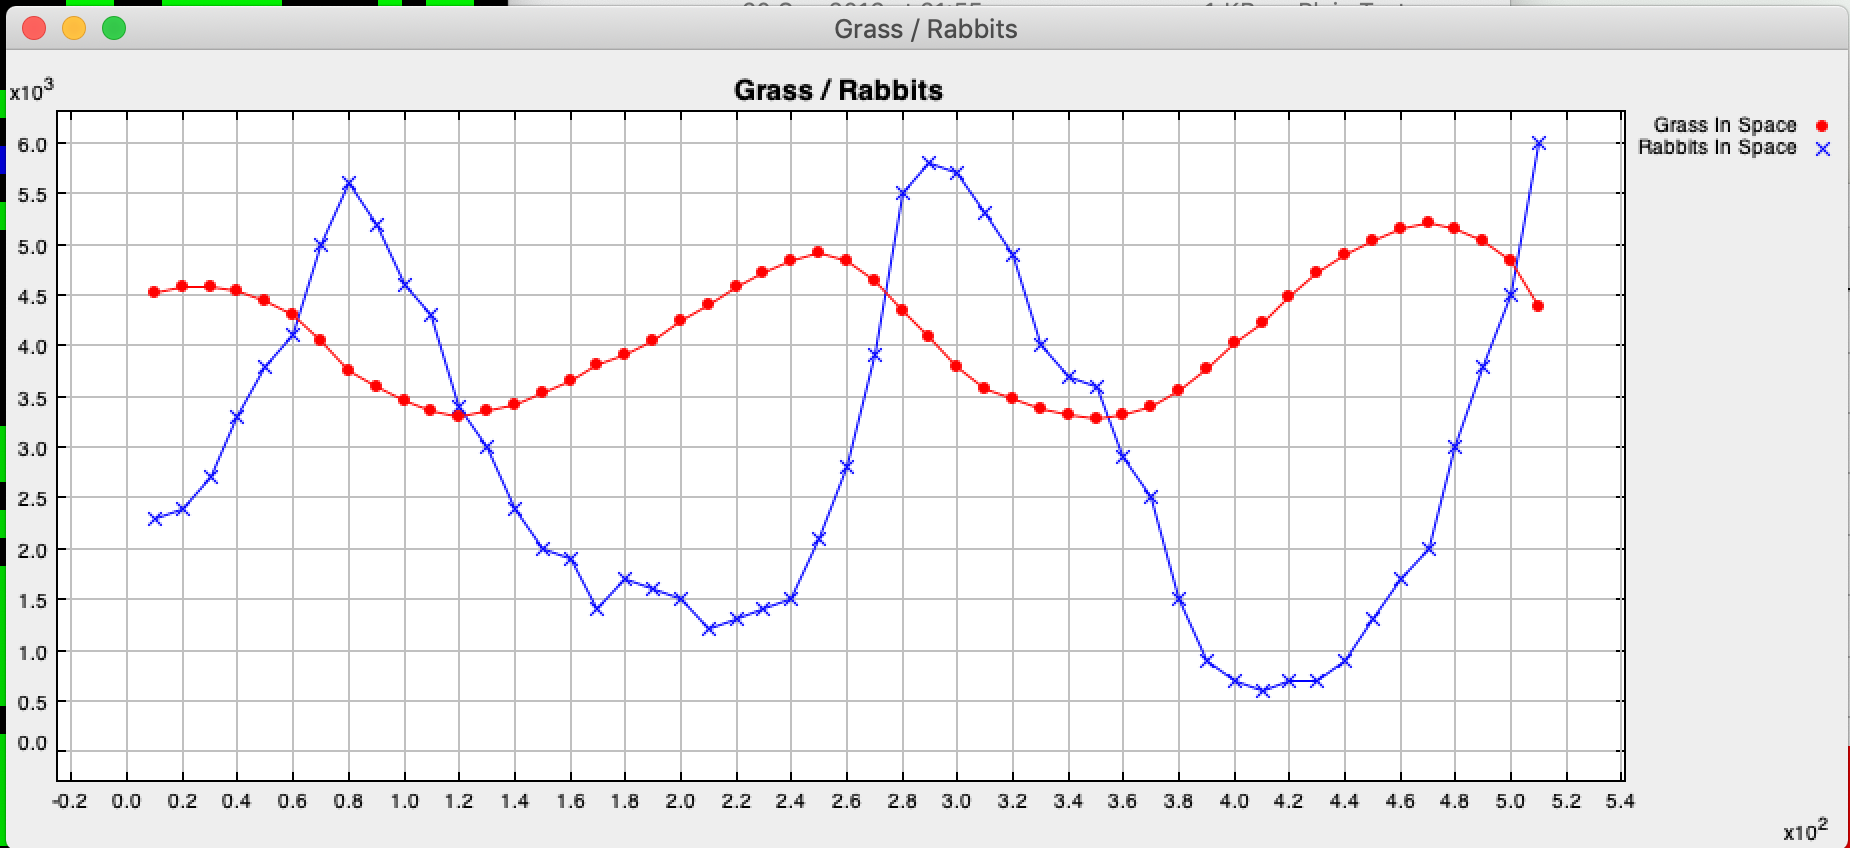
\includegraphics[width=\linewidth]{ex1-chart-20.png}
  \caption{20 rabbits}\label{fig:ex1-1}
\endminipage\hfill
\minipage{0.32\textwidth}
  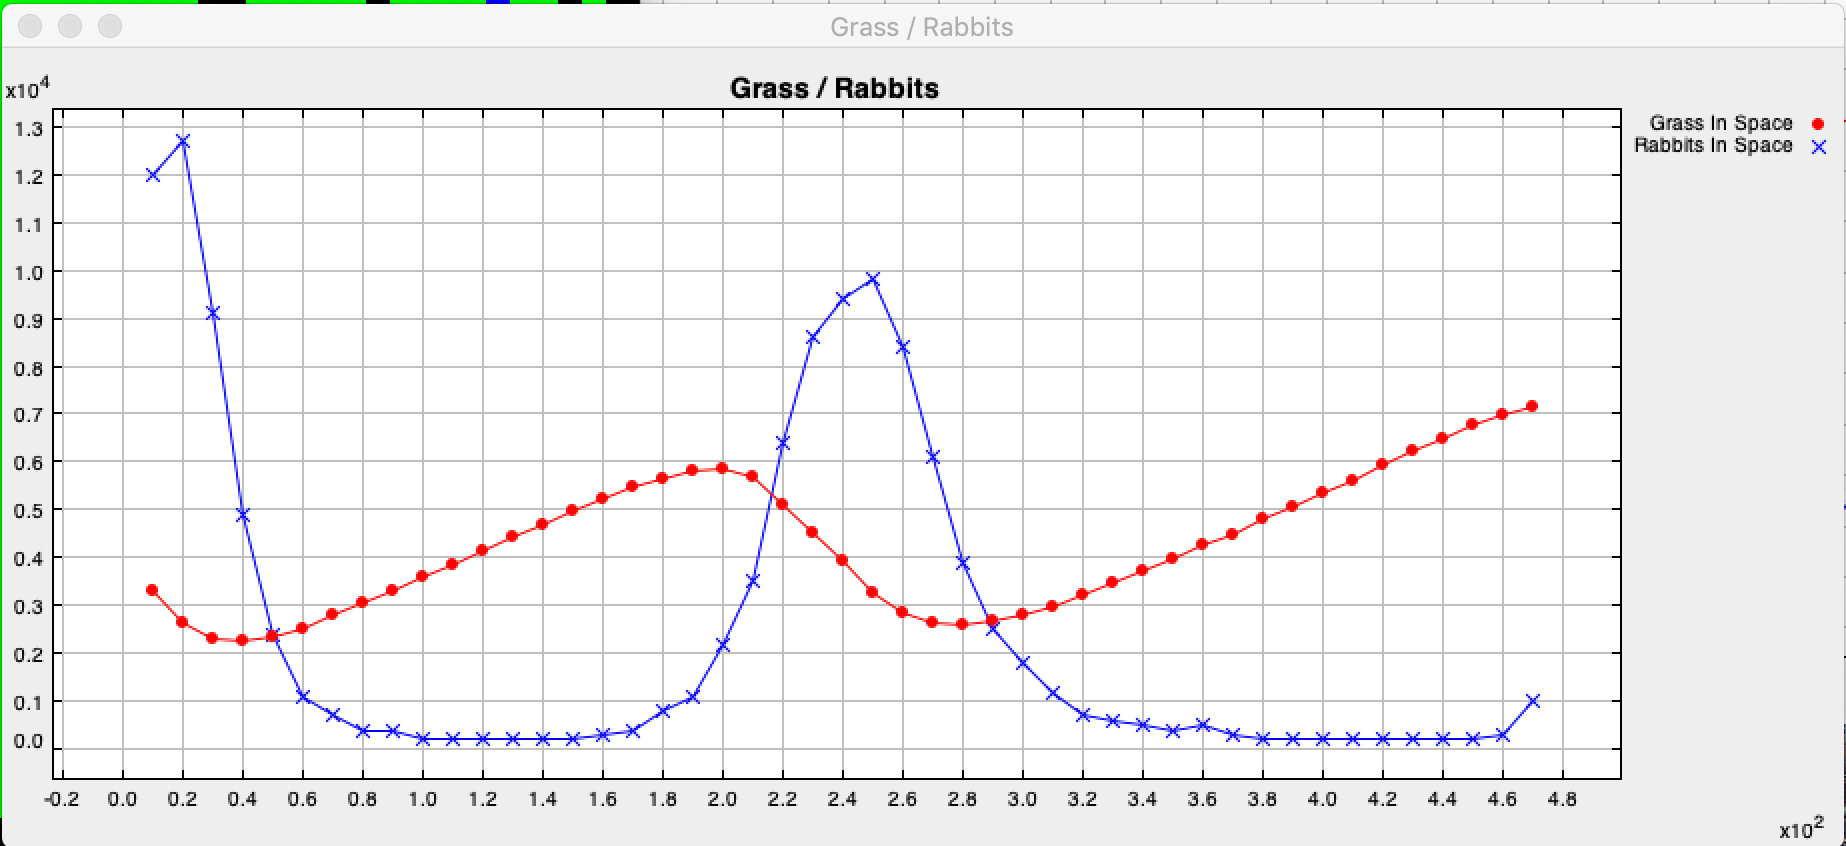
\includegraphics[width=\linewidth]{ex1-chart-100.png}
  \caption{100 rabbits}\label{fig:ex1-2}
\endminipage\hfill
\minipage{0.32\textwidth}%
  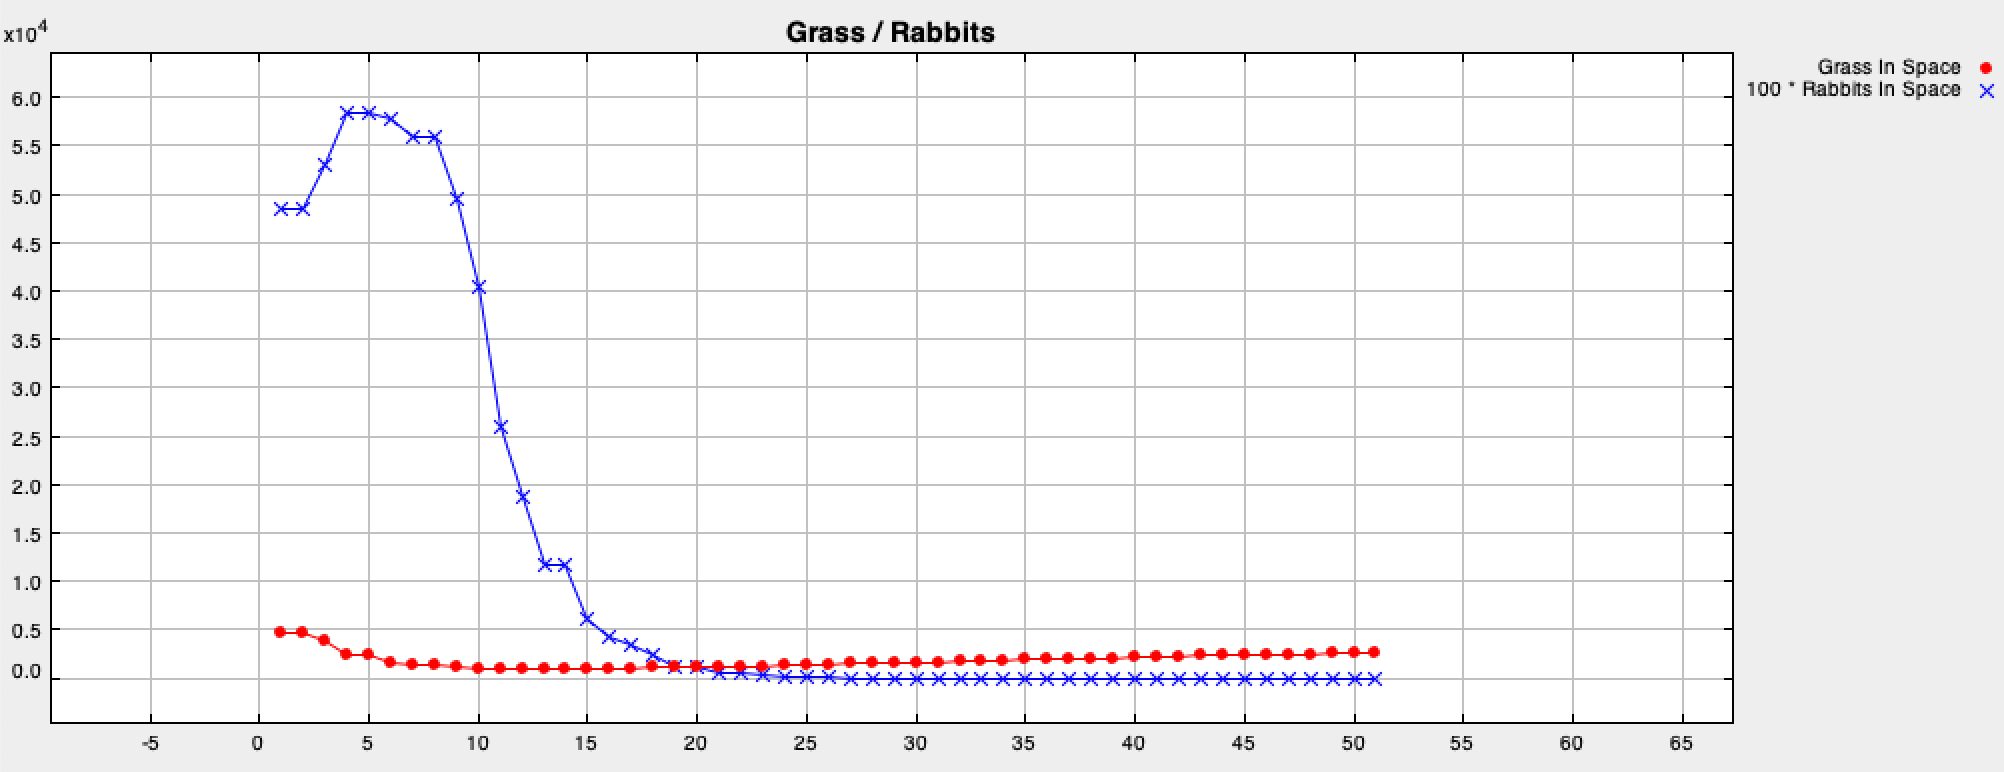
\includegraphics[width=\linewidth]{ex1-chart-300.png}
  \caption{300 rabbits}\label{fig:ex1-3}
\endminipage
\end{figure}

\subsection{Experiment 2}

\subsubsection{Setting}

Following our previous experiment, we decided to changed the growth rate of the grass and see how it impacts the whole population. The rabbit population size was 20 and we variate the grass growth rate to 20, 100 and 300.

\subsubsection{Observations}

When the population equals the grass growth rate, eventually they get extinct. However, we saw that for higher growth rates, the rabbits population will tends to have smaller variation (ie converge). We found this is true even if set different birth thresholds.

\begin{figure}[!htb]
\minipage{0.32\textwidth}
  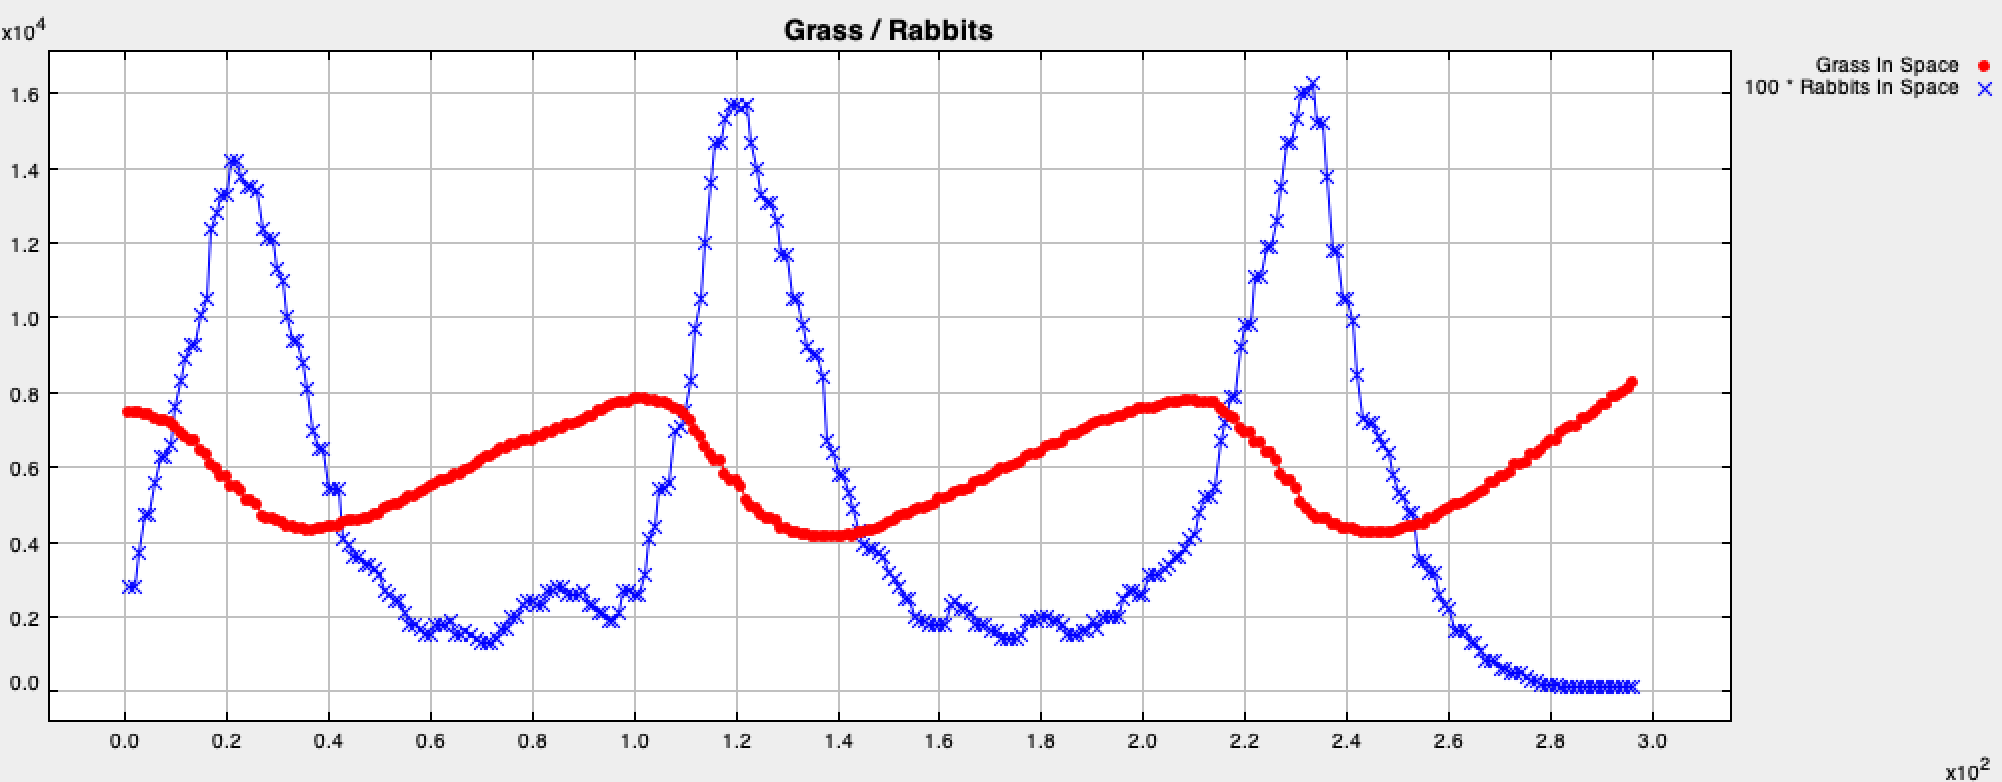
\includegraphics[width=\linewidth]{ex2-chart-20.png}
  \caption{20 growth rate}\label{fig:ex2-1}
\endminipage\hfill
\minipage{0.32\textwidth}
  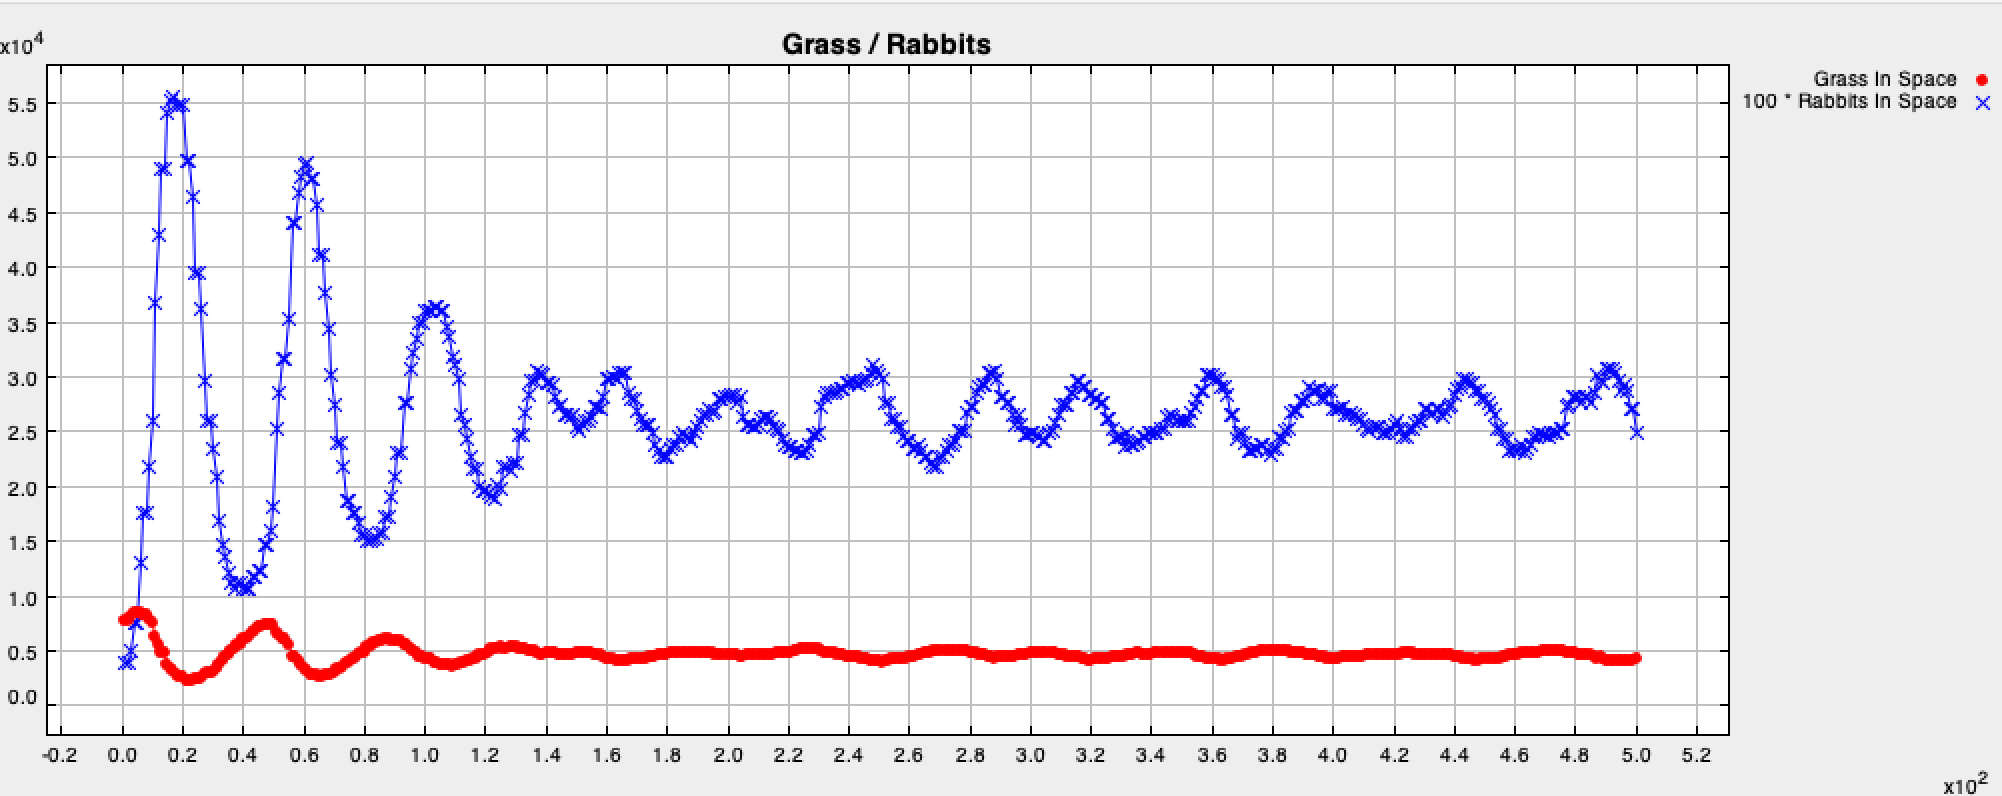
\includegraphics[width=\linewidth]{ex2-chart-100.png}
  \caption{100 growth rate}\label{fig:ex2-2}
\endminipage\hfill
\minipage{0.32\textwidth}%
  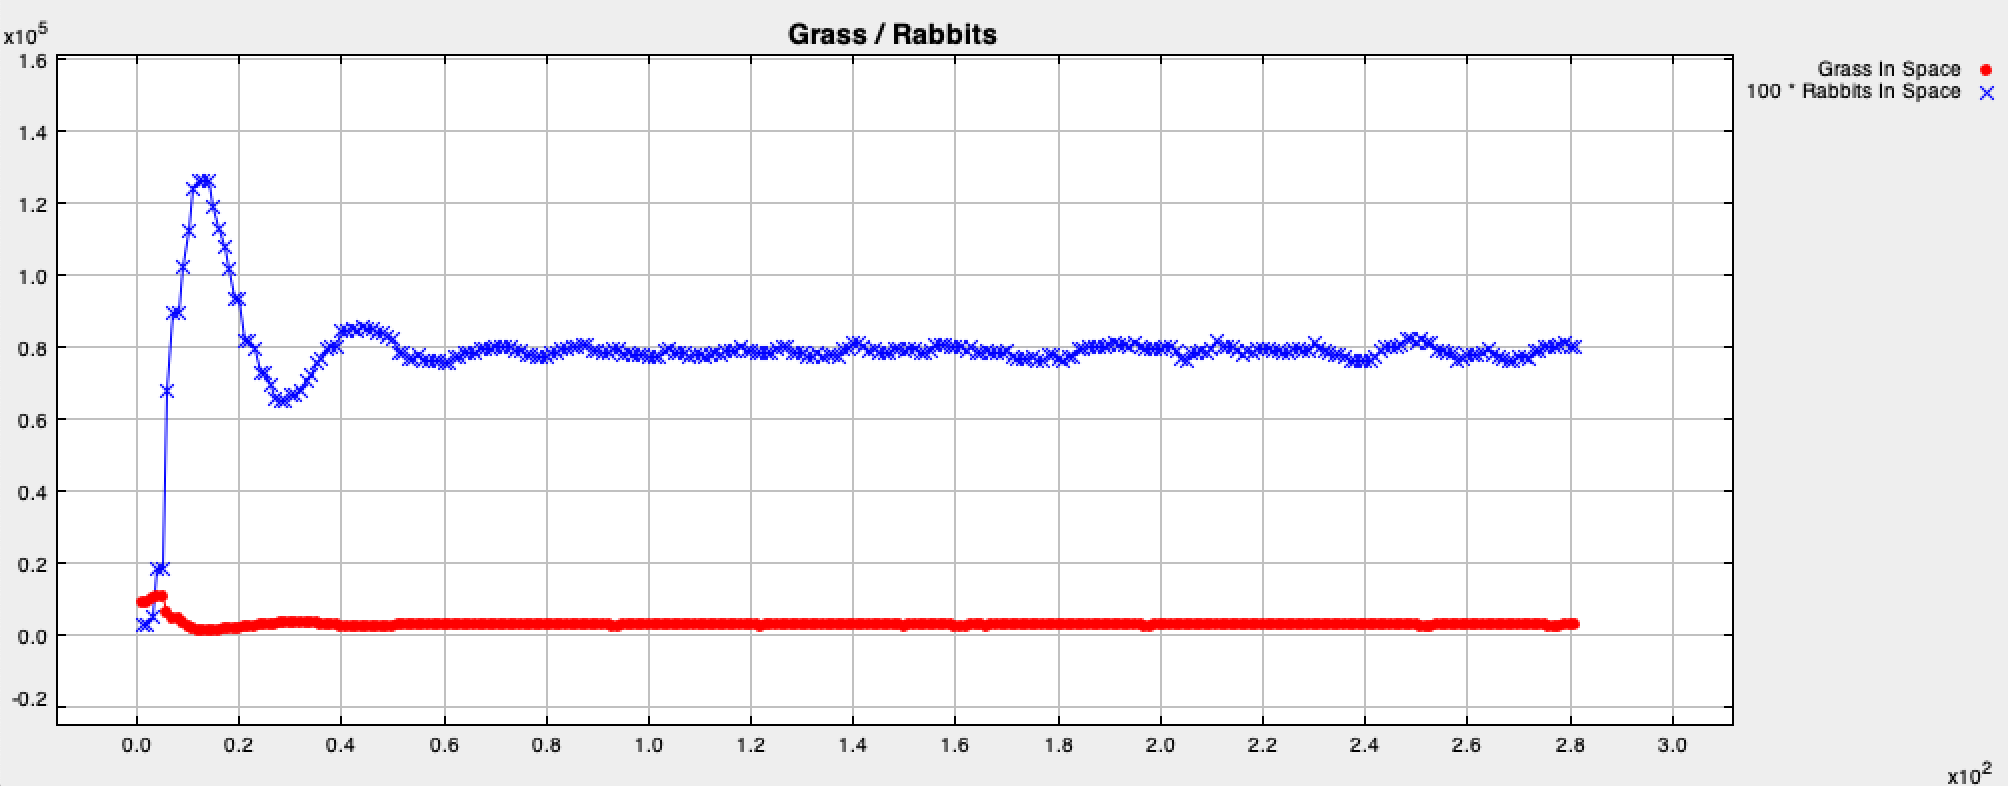
\includegraphics[width=\linewidth]{ex2-chart-300.png}
  \caption{300 growth rate}\label{fig:ex2-3}
\endminipage
\end{figure}


\subsection{Experiment 3}

\subsubsection{Setting}

Based on our previous experiments, we decided to change the birth threshold and the energy from eating a unit of grass. We used different values for this.

\subsubsection{Observations}

The behaviour of the population over the long term didn't affect the same patterns we saw previously. The population is still either converging or dying based on the growth rate of the grass.

\end{document}
